\chapter{Onderzoek: Methode en tooling voor SOUP-analyses}\label{ch:onderzoek-tool-methode}
In het vorige hoofdstuk is duidelijk geworden dat er veel externe bibliotheken worden gebruikt bij de ontwikkeling van applicaties. Veel bedrijven kunnen niet meer zonder en Eaglescience is hier geen uitzondering op. Het gebruik van externe bibliotheken biedt namelijk veel voordelen op het gebied van besparing (tijd en geld), flexibiliteit en standaardisering, ten opzichte van interne ontwikkelde bibliotheken.

Het gebruik van externe bibliotheken is echter niet zonder gevaren. Het is daarom zaak om, volgens de OWASP aangegeven manier, te controleren wat de staat is van de te gebruiken bibliotheken. Als dit niet gedaan wordt, bestaat de kans dat informatie wordt bemachtig of dat functionaliteit binnen een applicatie misbruikt kan worden door kwaadwillenden. Er bestaan bronnen zoals de National Vulnerability Database (NVD) van het National Institute of Standards and Technology (NIST) waarin deze kwetsbaarheden worden opgeslagen. Het is echter ondoenlijk om deze database met de hand te doorzoeken. Zeker op het moment dat applicaties dusdanig veel bibliotheken gebruiken dat het volume simpelweg te groot wordt. Volgens de aanwijzingen van OWASP top10 dienen alle dependencies en de geneste dependencies gecontroleerd te worden.
Dit onderzoek beoogt om tooling en methoden te identificeren voor Eaglescience om automatisch en periodiek SOUP-analyses te kunnen doen zodat kwetsbaarheden in applicaties inzichtelijk kunnen worden gemaakt. Door gebruik van deze methode hoeft alleen de applicatie nog met de hand up-to-date te worden gehouden. Dit laatste is door de complexiteit bewust uit de opdracht gehouden. Een bijkomend voordeel is dat er door de SOUP-analyse naast de kwetsbaarheden ook gegevens worden vastgelegd over de bibliotheken waardoor er in de toekomst een beter beeld bestaat over het gebruik daarvan. Dit beeld kan gebruikt worden om bij een gevonden kwetsbaarheid te achterhalen welke applicaties hier ook afhankelijk van zijn. Dit levert op zijn beurt weer een directere manier van onderzoek op.

De onderzoeksvraag is: $"$Welke Software Composition Analyses(SCA) tooling is compatibel met de omgeving van Eaglescience en welke methode kan worden toegepast om deze tooling te gebruiken voor het automatisch analyseren van externe dependencies?$"$. De hoofdvraag werpt de volgende deelvragen op, verdeelt in twee domeinen, die elk hieronder worden beantwoord in een eigen paragraaf waarna in de conclusie de methode wordt beschreven die geschikt wordt geacht als basis voor het ontwerp.
\begin{itemize}
    \item Huidige situatie binnen Eaglescience:
    \begin{itemize}
        \item Welke werkwijze en Dev-stack gebruikt Eaglescience voor het ontwikkelen van software?
        \item Hoe wordt er op dit moment software uitgerold binnen Eaglescience?
        \item Wat zijn de selectiecriteria voor tools die gebruikt kunnen worden?
    \end{itemize}

    \item Onderzoek om de huidige situatie binnen Eaglescience om te zetten naar de nieuwe situatie:
    \begin{itemize}
        \item Welke tools zijn er beschikbaar?
        \item Hoe zijn deze tools te integreren in de huidige buildstraat van Eaglescience?
        \item Welke methode kan worden gebruikt om middels de gevonden tools informatie over kwetsbaarheden binnen externe bibliotheken te vinden?
    \end{itemize}
\end{itemize}


\section{Werkwijze en dev-stack binnen Eaglescience}\label{sec:werkwijze-en-dev-stack-binnen-eaglescience}
Voordat er kan worden onderzocht welke tools en methode er geschikt zijn om een analyse te doen op projecten die Eaglescience in haar beheer heeft, dient er gekeken te worden naar de manier waarop Eaglescience werkt en met welke middelen projecten worden ontwikkeld. Deze kennis is nodig om een scope aan te brengen in de zoektocht naar tooling.


\subsection{Werkwijze}\label{subsec:ESwerkwijze}
Binnen Eaglescience wordt er geprobeerd om $"$full Scrum$"$ te werken. Dit wil zeggen dat voor ieder project een team van maximaal 9 full-stack ontwikkelaars wordt aangewezen. De sprints duren ongeveer 2 á 3 weken afhankelijk van wensen van de klant en beschikbaarheid van ontwikkelaars. Iedere sprint begint met een refinement door het team waarbij de taken die op de backlog staan worden bekeken en ingeschat. Tijdens de sprint vindt de ontwikkeling, opgedeeld in taken, plaats welke vervolgens worden gereviewd door een ander teamlid. Aan het einde van de sprint vindt er een retrospective plaats en een demo om de voortgang te demonstreren aan de klant. Daarnaast kunnen de projectmanager en product owner de taken die op de back-log staan opnieuw prioriteren, wat mee kan worden genomen in de volgende sprint.

\subsection{Dev-stack}\label{subsec:ESdev-stack}
Eaglescience maakt full stack oplossingen. Er worden dus zowel frontend, back-end, en database oplossingen ontwikkelt binnen projecten. Hierom wordt er binnen EagleScience gebruik gemaakt van verschillende ontwikkeltalen en tooling. Hieronder staan de belangrijkste vermeld.

\subsubsection{Ontwikkeltalen en frameworks}\label{subsubsec:ontwikkeltalen-en-frameworks}
Zoals eerder beschreven ontwikkelt Eaglescience software full-stack. Er wordt dus gebruik gemaakt van talen voor de frontend en back-end. Databases worden niet meegenomen in de lijst omdat deze als complete componenten worden gezien en de analyse op SOUP in deze ook niet veel zin heeft.
\begin{itemize}
    \item \textbf{Backend} De meest voorkomende taal binnen Eaglescience voor het ontwikkelen van de back-end binnen Eaglescience is Scala. Hiervoor is gekozen omdat deze taal de mogelijkheid biedt om functioneel te programmeren in de Java Virtual Machine (JVM). Hierdoor kunnen bibliotheken die geschreven zijn in talen die ook ondersteunt worden door de JVM gebruikt kunnen worden door Scala. Daarbij heeft Scala de mogelijkheid om naadloos mee te groeien met een project. Deze eigenschap komt bovendien terug in de naam Scala, wat een samenraapsel is van Scalable Language. De ondersteuning voor functioneel programmeren heeft als voordeel dat de geschreven code makkelijker te testen is, wat te danken is aan het juiste gebruik van pure functies. Pure functies hebben de eigenschap deterministisch te zijn, wat wil zeggen dat iedere keer als een bepaalde input in een functie komt er altijd dezelfde output verwacht kan worden, zonder dat er side-effects plaatsvinden die de staat van een applicatie onbedoeld kunnen veranderen. Dit komt de betrouwbaarheid ten goede. Deze eigenschap maakt het mogelijk om applicaties sneller en makkelijker te testen. Binnen Eaglescience worden er in bijna alle projecten een aantal frameworks/bibliotheken gebruikt die het ontwikkelen van microservice web applicaties in Scala makkelijker maken:
    \begin{itemize}
        \item \textbf{PlayFramework 2.xx} Een web framework voor de ontwikkeling van webapplicaties in Scala.
        \item \textbf{ArchES} Een intern ontwikkeld framework die de opbouw en communicatie tussen microservices in Scala verbeterd. ArchES is geïnspireerd op een message us systeem en werkt middels het pub → sub principe.
    \end{itemize} Binnen Scala kan er gebruik worden gemaakt van enkele buildtools zoals Maven, Gradle en Scala Build Tool (SBT). Binnen Eaglescience wordt SBT gebruikt omdat het de de facto tool is voor Scala.
    \item \textbf{Frontend}
    Voor de frontend wordt bij Eaglescience bijna altijd gebruik gemaakt van TypeScript, een extensie op Javascript. TypeScript maakt het mogelijk om in JavaScript getypeerd te programmeren wat mogeloijk maakt dat bugs en andere fouten tijdens het ontwikkelen opgemerkt worden, zodat deze niet pas tijdens run-time aan het ligt komen. Eaglescience gebruikt framework Angular het meest voor de ontwikkeling van de diverse portalen en User-interfaces. NativeScript wordt gebruikt in combinatie met Angular om Mobile apps te ontwikkelen. De reden voor het gebruik van Nativescript is dat het de mogelijkheid biedt om Angular te gebruiken voor de ontwikkeling van zowel android als IOS-apps. Beide ontwikkel frameworks draaien in JavaScript en om die reden wordt Node.js gebruikt als ontwikkelomgeving. Gezien JavaScript niet gecompileerd en dus niet gebuild wordt (zoals in Scala) is er alleen een voorziening voor dependency management in de vorm van Yarn en Node Package Manager (NPM). Binnen Eaglescience wordt NPM gebruikt voor het beheer van dependencies in een project.
\end{itemize}

\subsubsection{Tooling}\label{subsubsec:tooling}
Naast ontwikkeltalen gebruikt Eaglescience een aantal tools om dagelijkse werkzaamheden te stroomlijnen en software uit te rollen voor de klant. De tools zijn ieders verantwoordelijk voor een specifieke taak en alle projecten dienen, wanneer gepast, gebruik te maken van deze tools.

\begin{itemize}
    \item \textbf{Jira}
    Binnen Eaglescience wordt Jira gebruikt voor taakbeheer binnen projecten. Hier worden taken aan projecten toegevoegd welke vervolgens in een sprint worden opgenomen. Ook de sprints worden beheerd middels Jira.
    \item \textbf{Confluence}
    Confluence wordt gebruikt voor de documentatie van de verschillende projecten waar Eaglescience aan werkt. Confluence en Jira zijn beiden van Atlassian waardoor deze met elkaar kunnen communiceren, wat op zijn beurt de documentatie vereenvoudigd. Op dit moment lijkt het erop dat Confluence-server en Jira-Server een end of life heeft in 2023 en dat er hierdoor dus een vervanging moet worden gevonden.
    \item \textbf{GitLab}
    Gitlab wordt binnen Eaglescience gebruikt als Version control systeem. Er is gekozen om GitLab on premise te gebruiken op een server in eigen beheer op locatie. Gitlab biedt naast version control ook andere tooling aan die het mogelijk maken om vanuit GitLab te builden en/of uit te rollen, echter wordt dit binnen Eaglescience gedaan middels een andere tool genaamd Jenkins.
    \item \textbf{Jenkins}
    Jenkins is een open-source automation server die door Eaglescience gebruikt wordt om projecten te builden, testen, en deployen. Jenkins is gebouwd op een Java omgeving en is daarom uitermate geschikt om met gradle, Maven en SBT-projecten om te gaan. Daarnaast kan het middels diverse Shellscripts (Bash, SH, PowerShell) aanverwante taken uitvoeren. Als laatst kan het middels plugins ook uitrollen op cloud omgevingen. Om deze redenen heeft Eaglescience gekozen om Jenkins te gebruiken. In een sectie hieronder wordt uitvoerig uitgewijd over hoe Jenkins binnen Eaglescience een project build, test en uitgerold.
    \item \textbf{Portal}
    Eaglescience ontwikkeld momenteel een medewerkers portal welke tools en gegevens aan kan bieden die niet project specifiek zijn. Op dit moment wordt er een LDAP password reset tool en verlof inzage en aanvraag aangebonden. Er wordt naast de module voor SOUP-analyses ook een module ontwikkeld welke het mogelijk maakt om uren te registreren. Deze ontwikkelingen zijn een antwoord op de wens om systemen samen te voegen om zo een overzichtelijker geheel aan te kunnen bieden aan werknemers.
\end{itemize}

\section{Hoe wordt op dit moment software gedeployed?} \label{sec:hoe-wordt-op-dit-moment-software-gedeployed?}
Zoals hierboven is beschreven, wordt Jenkins gebruikt om de software te deployen. Het heeft de mogelijkheid om meerdere builds te doen voor verschillende projecten. Ieder project wordt op een eigen node gebouwd, waarbij de personal builds gehost worden op deze node. De development, en productie deploys gaan naar Azure in een specifiek ingericht cluster voor deze omgevingen.

Een deploy wordt gedaan op het moment dat er source code naar GitLab gepushed wordt. Door middel van Tokens in de commit message kan gestuurd worden waar de build (als deze slaagt) gedeployed wordt bijv: {-all + portal} build en deployed alleen de portal. [ci-skip] zorgt ervoor dat er alleen een push wordt gedaan en geen build wordt gestart.
Samengevat worden er dus parameters meegegeven in de commit op basis waarvan wordt besloten of er een build moet plaatsvinden en zo ja waar en voor welke delen van de applicatie. Op deze manier wordt er flexibiliteit aan de ontwikkelaar geboden. Een typische build en deploy gaat volgens figuur~\ref{fig:JenkinsPipeLine}.

\begin{figure}
    \myfloatalign
    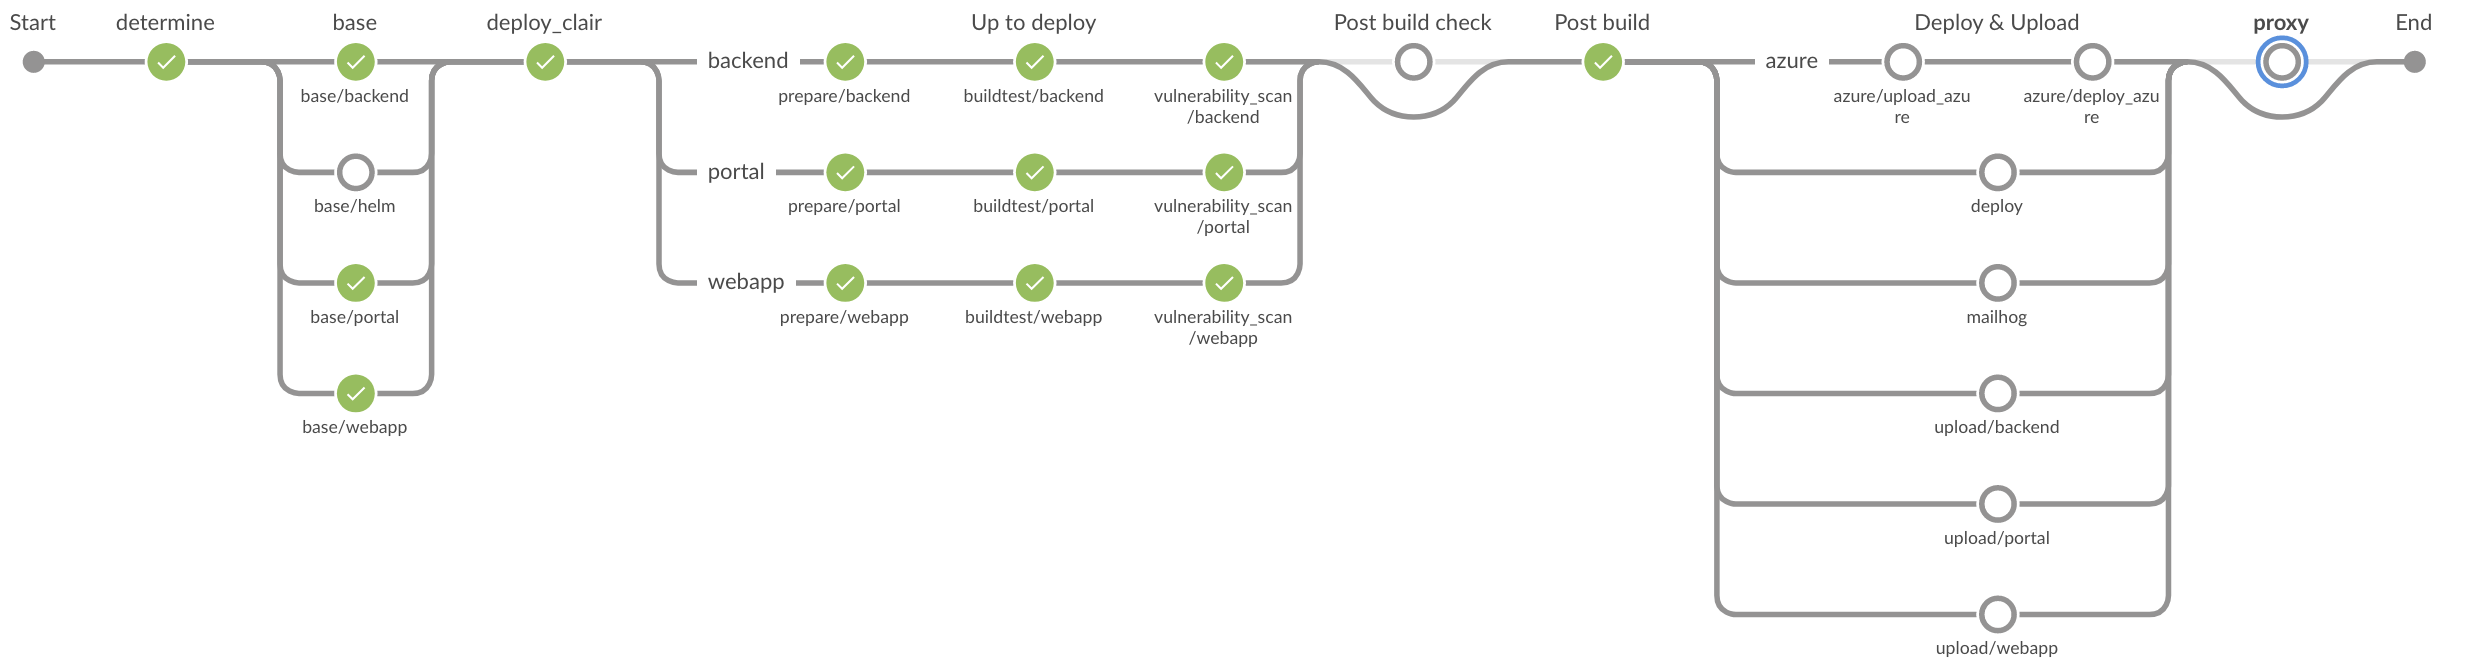
\includegraphics[width=12cm]{gfx/Screenshot 2021-08-18 Jenkins PipeLine}
    \caption{Jenkins(Blue Ocean) pipeline}
    \label{fig:JenkinsPipeLine}
\end{figure}
Een Jenkins pipeline werkt in een aantal stappen die in een .jenkinsFile worden beschreven, welke meegegeven wordt in een repository. Deze .jenkinsFile wordt in de determine stap ingelezen waarna de benodigde stappen op een rij worden gezet. Hieronder worden deze stappen in meer detail beschreven:
\begin{itemize}
    \item \textbf{determine} Hier wordt bekeken, aan de hand van een .jenkinsFile en tokens in de commit, welke stappen er nodig zijn om een succesvolle build en/of deploy te kunnen doen.
    \item \textbf{base} In de base stap worden alle images voorbereid die nodig zijn om de applicatie te builden. Images worden hier opgehaald waarna de containers worden voorbereid. De base stap is een parallel-lopende stap waarin, in het voorbeeld van het figuur, het Operating system, de backend, portal en de app  met de nodige bibliotheken worden voorbereid.
    \item \textbf{deploy clair} De clair scanner wordt hier opgestart waardoor het in een latere stap beschikbaar is om een scan uit te voeren op de gebouwde containers.
    \item \textbf{Up to deploy}
    In het voorbeeld van het figuur wordt er voor de backend, portal, en app een parallel process gestart waarin de volgende drie substappen worden doorlopen:
    \begin{itemize}
        \item \textbf{prepare} Docker containers worden ingesteld en klaar gezet voor het ontvangen van de services(Software en bibliotheken).
        \item \textbf{buildtest} De services worden gebuild en getest in deze stap. Eaglescience heeft een aantal thresholds opgesteld waaraan tests moeten voldoen. Om deze te analyseren worden de test resultaten vanuit de docker containers gekopieerd naar de Jenkins Store waar Jenkins de waarden kan analyseren. Als alle unit-tests binnen de resultaten vallen wordt de volgende stap uitgevoerd.
        \item \textbf{vulnerability scan} Clair scanner scant nu de containers nogmaals, maar nu op de in de applicatie benodigde software (run time environments, databases etc.). Als clair iets vindt dat Eaglescience als verdacht acht dan wordt de build gestaakt.
    \end{itemize}
    \item \textbf{PostBuild(check)}
    Alle bevindingen worden hier gecheckt en mocht er iets mis zijn wordt er wederom afgebroken en is de build gefaald en zal er dus geen deploy plaatsvinden.
    \item \textbf{Deploy \& Upload}
    In het voorbeeld opgenomen in het figuur wordt de deploy niet uitgevoerd. Deze stap zorgt ervoor dat de gebouwde containers worden overgedragen naar Azure. Iedere container heeft wederom zijn eigen stappen. De upload valt echter buiten de scope van dit onderzoek.
    \item \textbf{End}
    Einde van de PipeLine Jenkins geeft de workers die het project heeft gebruikt weer vrij.
\end{itemize}


\section{Passende Software Composition Analyses(SCA) tooling}\label{sec:sca-tooling}

In de opdracht staat vermeld dat de te ontwikkelen module eenvoudig in gebruik dient te kunnen worden genomen binnen de bestaande CI/CD Pipeline en dat de resultaten zichtbaar moeten zijn in de huidige portal. Hierom moet er dus Software Composition Analysis (SCA) tooling gevonden worden die makkelijk te integreren is in de huidige Jenkins pipeline, welke resultaten geeft die vervolgens te verwerken zijn tot een leesbare pagina in de portal. Als we deze stelling ontleden moeten er een aantal zaken worden onderzocht:
\begin{itemize}
    \item Welke tooling is er beschikbaar om SOUP-analyses uit te voeren op zowel SBT (Scala) als NPM (Node.js)-projecten?
    \item Welke resultaten worden er door de tool geproduceerd?
    \item Hoe kan de tooling worden geintegreerd in de huidige Jenkins pipeline?
\end{itemize}
Om deze vragen te beantwoorden moet er eerst geschikte tooling gevonden worden die, bij voorkeur, met zowel SBT als NPM-projecten overweg kan. Vervolgens dient er gekeken te worden naar hoe de geselecteerde tooling een resultaat bouwen, hoe deze eruit ziet en in welke tijd het resultaat gegeven kan worden.

\subsection{Tooling: Welke tooling is beschikbaar om SOUP-analyses uit te voeren op zowel SBT (Scala) als NPM (Node.js)-projecten?}\label{subsec:ESTooling}
Er zijn een aantal bedrijven en instanties die tooling aanbieden om analyses te doen. Een google search op $"$Scala dependency scan$"$ levert op de eerste resultaten pagina direct Snyk.io, SonarSource en OWASP op.

Snyk is een tool die geschikt is om Scala en TypeScript code, en dus bibliotheken te analyseren. Snyk kan worden ingezet op zowel SBT als NPM-projecten. Het biedt voor de analyse van code meerdere opties. Eén van die opties is middels een CLI Tool welke rapporteert naar een Dashboard gehost door Snyk zelf. Een andere optie die Snyk aanbiedt is te scannen middels een plugin via InteliJ, welke door Eaglescience gebruikt wordt. Als laatste optie biedt Snyk een plugin voor Jenkins die te integreren is in de buildstraat van Eaglescience. De voordelen van Snyk zijn dat er een volledig pakket wordt geboden, waarbij ook nog andere veiligheidsaspecten kunnen worden gecontroleerd (zoals het scannen van zelf geschreven code). Echter, om de volledige functionaliteit van Snyk te kunnen benutten is er een licentie nodig. Het nadeel hiervan is dat dit op periodieke basis geld kost. Een ander nadeel is dat de resultaten in een eigen omgeving, welke extern gehost wordt, kan worden ingezien. Hierdoor valt deze tooling echter buiten de vooraf gestelde criteria.

SonarSource is een ander bedrijf dat tooling aanbiedt voor het analyseren van source-code. Het doet dit door in de verschillende stadia van het proces tooling aan te bieden die helpen de kwaliteit van geleverde applicaties te verhogen. Als eerste biedt het een gratis plugin aan (SonarLint) voor verschillende IDE's waarbij actief wordt gekeken naar fouten, bugs en dergelijken tijdens het schrijven van code. Op die manier wordt er gekeken of code volgens standaarden worden geschreven en er geen kwetsbaarheden worden toegevoegd. Daarnaast is er een pakket dat SonarQube heet. Dit pakket biedt de mogelijkheid aan om op verschillende momenten naar de kwaliteit en de veiligheid van de aanwezige code te kijken. Hoewel SonarQube geschikt is om Scala en Typescript code te analyseren, is de SonarLint plugin niet compatibel met Scala code, maar wel met JavaScript en TypeScript. Er zijn meerdere versies beschikbaar die elk een specifiek aantal functionaliteiten aanbieden. Zo is er een community edition, welke gratis is, die als server geïnstalleerd kan worden en waar verschillende repositories kunnen worden bijgehouden. Hiernaast zijn er andere editions beschikbaar waarvoor betaald moet worden en er extra functies worden geleverd, zoals GitLab integration en dergelijke. Samengevat zijn de voordelen van SonarSource tooling dat er tijdens alle stadia van softwareontwikkeling controles worden ingebouwd die de code analyseren op o.a. kwetsbaarheden. Hiernaast kan SonarQube on premise draaien. Echter, een nadeel van de SonarQube plugin is dat SBT niet zelf door SonarSource ontwikkeld wordt, en SonarLint geen ondersteuning biedt voor SBT. De incompatibiliteit met Scala maakt integratie in de Eaglescience pipeline niet voor de hand liggend.

In eerdere onderzoeken is naar boven gekomen dat de OWASP zich bezig houd met het veilig houden van geschreven software. Een van de projecten die de OWASP aanbiedt is $"$Dependency-check$"$. Dit is een Software Composition Analysis (SCA) Tool die het mogelijk maakt om openbaar gemaakte kwetsbaarheden te detecteren door te kijken of er voor dependencies een Common Platform Enumeration (CPE) bestaat. Als deze CPE bestaat kan er gekeken worden of er een CVE voor bestaat en vervolgens worden weergegeven in resultaten. Als geen van beiden bekend is wordt er door de tool vanuit gegaan dat er op het moment van checken geen kwetsbaarheid gevonden is. Hoewel dit op het oog een goede tool is om SOUP te analyseren, is de in het project ontwikkelde versie niet geschikt om te scannen op SBT en NPM dependencies. Op de website van het project is echter een link naar een versie die SBT-projecten kan analyseren. Uit de NPM repository blijkt dat er een soortgelijke tool bestaat om NPM-pakketten te analyseren.

De SBT dependency check en de OWASP dependency check (scanner voor NPM) lijken op dit moment de meest voor de hand liggende tooling voor de SOUP-analyse. Beide tooling zijn gratis beschikbaar en open-source. Echter zijn dit geen op opzichzelfstaande tools, maar bieden ze wel de mogelijkheid om te worden geïntegreerd in suits zoals Snyk en SonarQube. Het feit dat ze losse tools zijn maakt het mogelijk om deze in te zetten in de buildstraat van Eaglescience. Een ander voordeel is dat beide tooling gebruik maken van dezelfde engine.


De tooling die geselecteerd is maken beide gebruik van de dependency-check engine uit het OWASP project.
De engine genereert een rapport door de beschreven dependencies te voorzien van een CPE. Deze CPE wordt vervolgens door de CVE-database van het NIST gehaald. Als er zowel een CPE als een CVE gevonden wordt dan is er een kwetsbaarheid gevonden. Mocht een CPE missen dan gaat de tool ervan uit dat er geen kwetsbaarheid gevonden is. Om performance te verbeteren wordt er iedere 4 uur een update gehaald van de database en deze lokaal opgeslagen, waarbij deze lokale database wordt gebruikt. Na 4 uur wordt de database opnieuw geupdate om er op die manier voor te zorgen dat deze up-to-date is. Deze interval is in te stellen in de configuratie van de engine.

%
%https://github.com/etnetera/owasp-dependency-check for Node.js /NPM
%https://github.com/albuch/sbt-dependency-check for SBT
%
%https://github.com/eliasgranderubio/dagda niet zelfde als OWASP maar wellicht usefull

\subsection{Testen van Tools}\label{subsec:testen-van-tools}

Het lijkt voor de hand te liggen dat zowel de SBT-dependency-check en de OWASP-dependency-check (NPM) verantwoorde keuzes zijn om verder te onderzoeken. Echter dienen deze eerst te worden onderzocht op bruikbaarheid voordat er kan worden gedacht aan implementatie. Om de bruikbaarheid te testen zijn de volgende scenario's opgesteld die samen een idee moeten geven over de werking binnen een project en toepasbaarheid binnen een methode die in de volgende sectie zal worden onderzocht.

Er is gekozen voor twee scenario's:
\begin{enumerate}
    \item \textbf{Bestaand Eaglescience Project} Om te achterhalen hoe de dependency check tools kunnen worden ingezet in projecten die op dit moment ontwikkeld en gehost worden, moeten de tools worden geïntegreerd in een bestaand project. Als project is gekozen voor GroeiGids\footnote{GroeiGids is op het moment van schrijven één van de grootste projecten waar Eaglescience aan werkt wanneer wordt gekeken naar code-volume en aantal dependencies. Het is een project in opdracht van de GGD en biedt ouders de mogelijkheid om groei informatie van hun kinderen in op te slaan.}, een van de grotere projecten waar op dit moment aan wordt gewerkt. Het project bevat zowel een frontend (NPM Angular) als een App (NPM NativeScript), evenals een uit microservices bestaand SBT-project (geschreven in Scala)Voor GroeiGids worden dependencies in een aparte file gedeclareerd en deze worden vervolgens geïmporteerd in de build.sbt. Theoretisch gezien zou dit geen probleem moeten zijn gezien SBT zelf ook gebruik maakt van deze constructie.

    \item \textbf{Alleen de dependency declaraties} Door alleen dependency declaraties te gebruiken in een test, en dus niet het volledige project, kan worden onderzocht of de geselecteerde tooling hiermee om kan gaan. Dit zou wenselijk kunnen zijn om op een ander moment een analyse uit te voeren op de verschillende projecten. Het zou op die manier ook periodieke controle op kwetsbaarheden mogelijk maken zonder dat er toegang is tot de source code.
\end{enumerate}

\subsubsection{Test 1a: SBT dependency scanning in een bestaand project}
\textbf{Doel:} Onderzoek naar het gebruik van de SBT-dependency-check plugin in GroeiGids. Het gewenste resultaat is kennis over hoe de plugin wordt geconfigureerd om de gewenste output, bij voorkeur een JSON-file/object, te verkrijgen. Daarnaast wordt beoogd om inzicht te krijgen in hoeveel tijd de plugin nodig heeft voor het genereren van het rapport.

\textbf{Methode:} Als eerste dient de SBT-dependency-check plugin te worden geïnstalleerd in het project middels de documentatie van het project. Vervolgens dient de output format te worden aangepast: \texttt{dependencyCheckFormats in Global += $"$JSON$"$}
en \texttt{dependencyCheckFormats in Global += $"$HTML$"$}. HTML wordt alleen gebruikt om in de test leesbare output te verkrijgen zodat deze kan worden geverifieerd met andere bronnen. Deze rapporten die resultaat zijn van het draaien van \texttt{SBT dependencyCheck} dienen te worden gecontroleerd tegen een andere bron. Daarnaast dient te worden bepaald hoeveel langer de analyse duurt wanneer de database wordt geupdate.

\textbf{Resultaat:} De analyse duurt ongeveer 173 seconden inclusief het ophalen/updaten van de database. Op het moment dat de database up-to-date is duurt een analyse 87 seconden. Dit zou dus inhouden dat een deploy 3 minuten langer duurt wanneer een SOUP-analyse wordt gedraaid voor een SBT project.
\begin{figure}
    \myfloatalign
    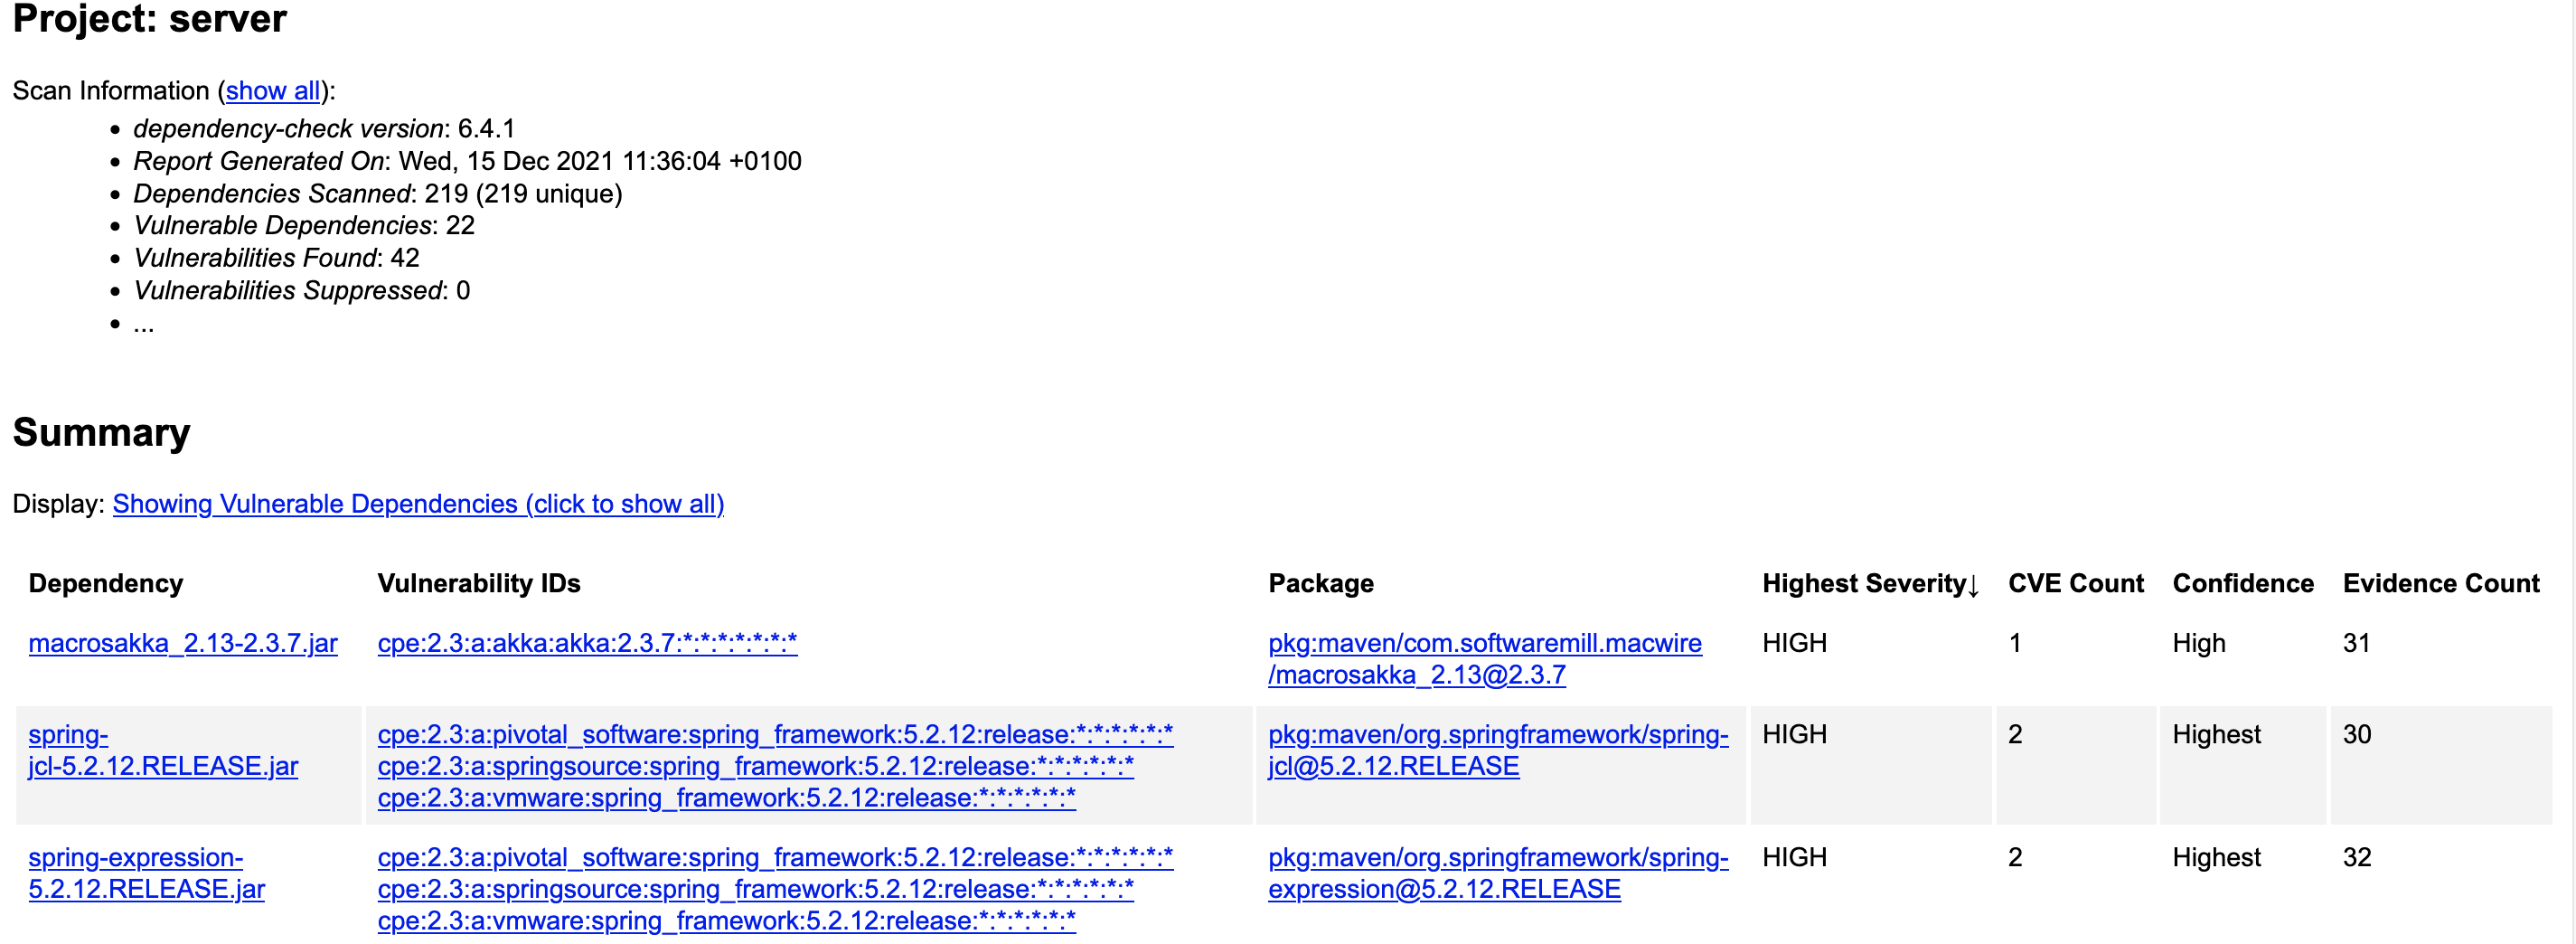
\includegraphics[width=15cm]{gfx/report_analyse_test1a_SBT}
    \caption{Deelresultaat van een analyse op de backend van GroeiGids}
    \label{fig:SBTReport1A}
\end{figure}

In figuur~\ref{fig:SBTReport1A} is te zien dat er 219 unieke dependencies gescanned zijn en dat er 42 kwetsbaarheden gevonden werden in 22 van de gescande dependencies. Na verificatie van de bovenste 5 vermeldingen tegen andere bronnen (openCVE), bleek dat deze overeenkwamen, en het vertrouwen wordt daardoor gewekt dat de analyse correct is.

\subsubsection{Test 1b: NPM dependency scanning in een bestaand project}

\textbf{Doel:} Onderzoek naar de algemene werking van de geselecteerde plugin, waarbij vooral gekeken moet worden naar welke instellingen er relevant zijn en/of de output nagenoeg overeenkomt met die van de SBT-analyse. Daarnaast moet de timing worden opgenomen.

\textbf{Methode:} Voor NPM bestaat er geen plugin, welke wel beschikbaar is voor SBT-projecten. Echter kan de OWASP-dependency-check worden toegevoegd als een dev-dependency \texttt{npm install -D owasp-dependency-check}, waarna er een script moet worden aangemaakt in package.json die het volgende aanroept \texttt{$"$owasp-dependency-check --project ''GroeiGids APP'' -f JSON -f HTML -o ''./reports'' ''}. De tag HTML is hierin op genomen om de leesbaarheid te vergroten voor de peer-review.

\textbf{Resultaat:} De output van deze analyse is nagenoeg gelijk aan die van de hierboven uitgevoerde analyse op SBT. De output van de check ziet er qua opmaak hetzelfde uit als die van SBT. Ook de verificatie met OpenCVE is goed dus ook hier is er het vertrouwen dat de correcte resultaten worden weergeven. Daarnaast duurt de scan zonder update van de database 21 sec en 139 seconden met een update van een database, zie figuur~\ref{fig:NPMReport1b}.

\begin{figure}
    \myfloatalign
    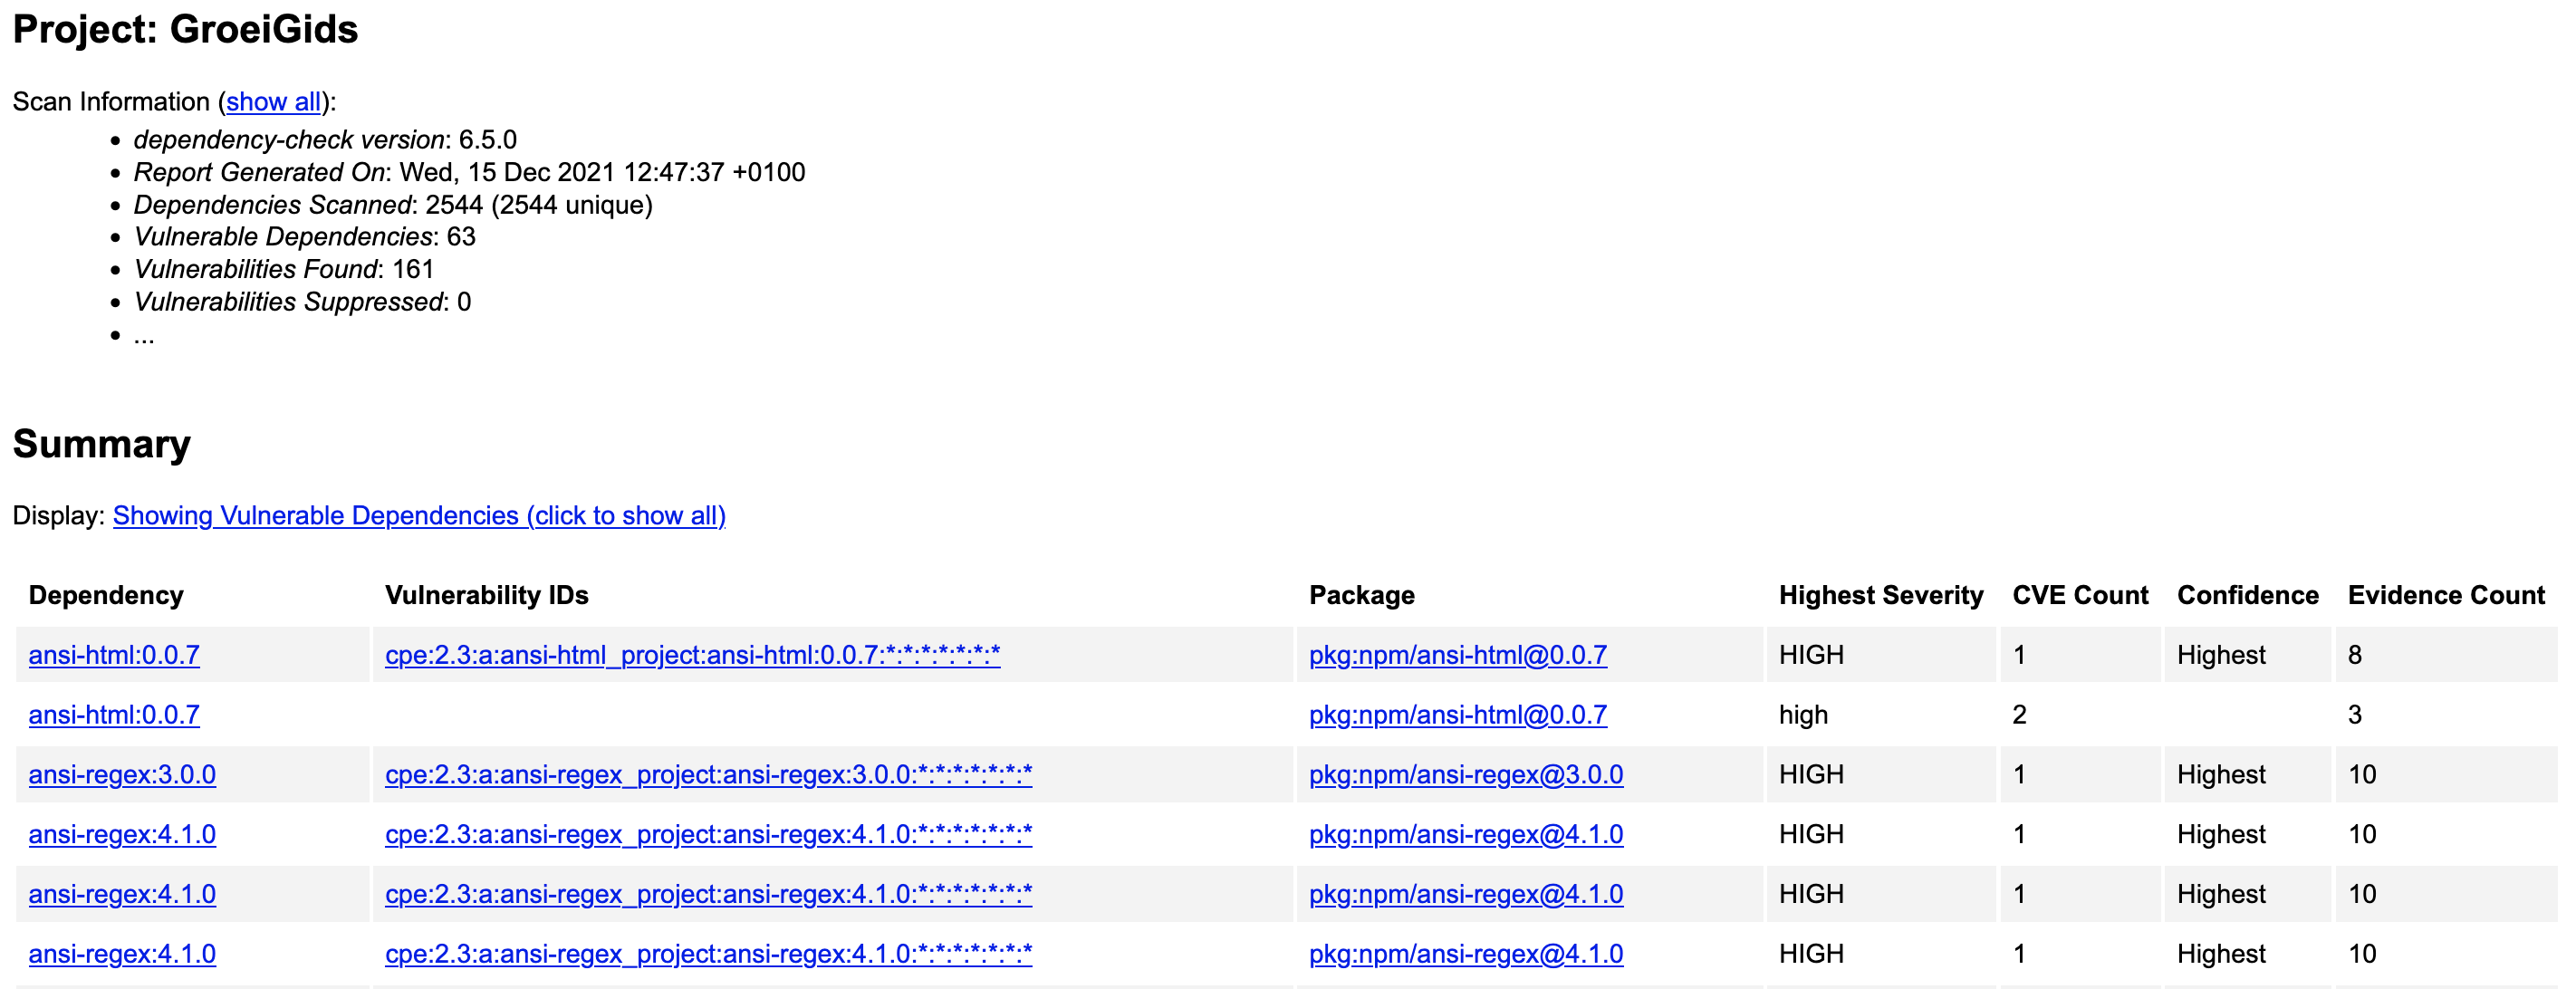
\includegraphics[width=15cm]{gfx/report_analyse_test1b_NPM}
    \caption{Deelresultaat van een analyse op de app van GroeiGids}
    \label{fig:NPMReport1b}
\end{figure}

Samengevat geven beide tools dezelfde rapporten conform hetzelfde JSON-schema. Het feit dat deze overeenkomen biedt mogelijkheden voor het ontwikkelen van een enkele procedure voor het opnemen van deze rapporten in de API.
Wanneer de tijden van het scannen van de SBT en NPM bij elkaar worden opgeteld duurt de analyse 108 sec wanneer de database niet wordt geupdate. Wanneer dit wel het geval is duurt de test 208 sec.

\subsubsection{Test 2a: SBT alleen de dependency informatie gebruiken}
Om te onderzoeken of een dependency check ook uitgevoerd kan worden zonder dat er een heel project bestaat en alleen een declaratie van dependencies in de build.sbt file staat wordt er een 2e test uitgevoerd.

\textbf{Doel:} Achterhalen welke bestanden er nodig zijn om een succesvolle analyse te doen. De uitkomsten moeten worden gecontroleerd op gelijkheid om te verifieren of deze methode dezelfde output genereert als in tests waarbij ook de source-code beschikbaar is.


\textbf{Methode:} Het GroeiGids project, welke gebruikt is voor de vorige test, wordt volledig gekopieerd naar een aparte folder, waarna alle source-code (incl. de bijbehorende mappen) wordt verwijderd. Het enige dat overblijft is de projectfolder met daarin een plugins.sbt waar de dependencyCheck is gedefinieerd, de dependencies.scala in de server folder en de build.sbt in de root. Vervolgens wordt de plugin gestart middels \textt{sbt dependencyCheckAggregate} en het resultaat in JSON vergeleken met het resultaat uit test 1a.

\textbf{Resultaat:} De rapporten die uitgegeven worden door zowel de eerste als de tweede test op het SBT-project zijn gelijk. De scantijden zijn ongeveer hetzelfde, wat aangeeft dat deze methode van scannen een goed alternatief is voor het scannen van projecten, en ook gebruikt kan worden voor het periodiek scannen van een project. Van belang zijn de volgende bestanden: plugins.sbt, build.sbt en dependencies.scala omdat hier de dependency check plugin wordt gedefinieerd, als ook plugins benodigd voor het project. In build.sbt en dependencies.scala worden dependencies gedeclareerd.

%TODO naar resulaten sectie kijken

\subsubsection{Test 2b: NPM alleen de dependency informatie gebruiken}
%Node.js docker container opzetten..
%package.json / package-lock.json copiere
%npm ci
%owasp script draaien
%cp resulst naar buiten
%destroy Container

Om te testen of de dependency check zonder informatie over het gebruik van de dependencies kan functioneren wordt er op eenzelfde manier getest als bij test 2a, maar dan voor NPM-projecten.

\textbf{Doel:} Onderzoeken wat er nodig is om een dependency check uit te voeren zonder source-code. Het vermoeden bestaat dat package.json en package-lock.json voldoende informatie bevatten om dit volgens verwachting uit te voeren. Daarnaast moet er gekeken worden of de packages geïnstalleerd dienen te worden.

\textbf{Methode:}
\texttt{NPM init} zal worden gebruikt om een nieuw leeg project op te zetten. Vervolgens moeten de dependency declaraties worden gekopieerd; package.json en package-lock.json.

Hierna wordt de dependency check toegevoegd aan package.json middels \texttt{npm -D install owasp-dependency-check}. Hierna moet er een \texttt{NPM ci} worden uitgevoerd om de declaraties in package-lock.json te installeren. Dit resulteert in een project zonder source-code, maar met geïnstalleerde dependencies zoals ze het laatst bekend waren (bijv tijdens deploy).

Vervolgens kan er middels een in package.json gedefinieerd script:\\ \texttt{''owasp'': ''owasp-dependency-check --project '' angularSandbox '' -f JSON -l ''dep-check-log.txt'' $"$}%TODO quotes goedzetten
een rapport worden gegeneerd, dat vergeleken kan worden met de uitkomsten van test 1b.

\textbf{Resultaat:}
Er kan enkel een analyse gedaan worden op het moment dat er zowel een package.json bestaat (declaratie van het script) als een package-lock.json (feitelijke dependency definitie van een laatste install), daarnaast dienen ook de dependencies te zijn geinstalleerd. Kennelijk is dit een vereiste vanuit de OWASP dependency check. In de logs zijn ook statements te vinden die erop wijzen dat niet geïnstalleerde dependencies worden geskipped\\
\texttt{2021-12-13 15:08:36,500\\
org.owasp.dependencycheck.analyzer.NodePackageAnalyzer:292\\
WARN  - dependency skipped: node module esbuild-darwin-arm64 seems optional and not installed}.\\

%De NPM Dependency check voert onderwater het volgende commando uit \texttt{/dependency-check.sh --out=./dependency-check-reports --project angularSandbox -f JSON --data=/tmp/dependency-check-data --scan=package-lock.json
%} de -f en de --out flags zijn de output flags die aangeven dat er een JSON file in depende-check-reports directory in de base gemaakt moet worden. --scan = package-lock.json is het bestand wat geacanned wordt wat wil zeggen dat er een node_modules folder moet zijn is aangemaakt middels een npm install op de package.json van het project.

\subsubsection{Conclusie tests}
Een analyse voor een project zo groot als GroeiGids duurt in het slechtste geval ongeveer 4 minuten. Hierbij is geen rekening gehouden met andere taken die processor tijd vragen. Deze tijd zal oplopen op het moment dat de Jenkins Server meerdere builds aan het uitvoeren is voor meerdere projecten. Echter, zijn de rapporten in zowel test 1 als test 2 gelijk dus kunnen we beide manieren gebruiken voor de ontwikkeling van een methode.


\newpage


\section{Methode voor extractie, verwerken en het publiceren van de resultaten gevonden in de projecten van Eaglescience}\label{sec:methodesoupes}

Er moet een methode worden ontwikkeld die in staat is om door de buildstraat gegenereerde gegevens te gebruiken voor het opbouwen van een rapport die in de portal te lezen is.
Deze methode moet op twee manieren werken:
Ten eerste moet het een dependency check uitvoeren tijdens het uitrollen om een rapport aan te kunnen bieden op het moment van deploy in Azure. Daarnaast moet het ook gegevens over het project zoals de dependency declaraties, project en build meta klaarzetten in een scan queue, zodat hiervan op een later moment gebruik van kan worden gemaakt.

De details van deze methode worden hieronder beschreven.


In figuur~\ref{fig:methodeSOUPanalyse} is de methode voor de SOUP-analyse uitgewerkt voor NPM en SBT. Voor beiden gelden globaal dezelfde stappen. Er zijn twee momenten waarop nuttige informatie kan worden verkregen uit de pipeline wanneer hieraan functionaliteiten worden toegevoegd ten behoeve van SOUP-analyse. Ten eerste is dit de \texttt{Vulnerability\_scan} stap, en ten tweede de \texttt{post\_build} stap. In de \texttt{Vulnerability\_scan} stap is de module gereed en kan deze gescaned worden op vulnerabilities. Door hieraan de dependency check toe te voegen kan er een rapport gegenereerd worden die in de Jenkins artifacts wordt opgeslagen. In deze stap wordt in dezelfde Jenkins artifacts ook de dependency declaraties opgeslagen voor dezelfde module.

Op dit moment is bekend welke dependencies er gebruikt worden en is er een check uitgevoerd. Om erachter te komen voor welk project dit is dient er in de post build stap metadata toegevoegd te worden die helpen bij de identificatie van het project. De projectmetadata omvat o.a. project naam, URL van de repo en welke modules het project bevat. De build metadata bevat o.a. \ de timestamp van de build, het resultaat van de build en welke githash er gebuild is. Deze metadata wordt ook in de Jenkins artifacts opgeslagen. Daarna worden alle artifacts gepost naar de SOUP API.
De SOUP API haalt hieruit de SBT (sbt-report.json) en NPM (npm-report.json) rapporten gegenereerd door de dependency check. Vervolgens worden hieruit de relevante data gefilterd door de report builder, welke het daarop in een database plaatst die door de portal gebruikt kan worden.


Om periodiek te kunnen scannen, worden de project en de build metadata samen met de dependency declaraties als een snapshot in een scan que gezet. Deze scan que kan periodiek worden doorlopen, om de projecten die hierin staan te scannen op kwetsbaarheden waarvoor de dependency check gebruikt wordt. Via de report builder zullen hiervan de resultaten in de database worden geplaatst.

\begin{figure}
    \centering
    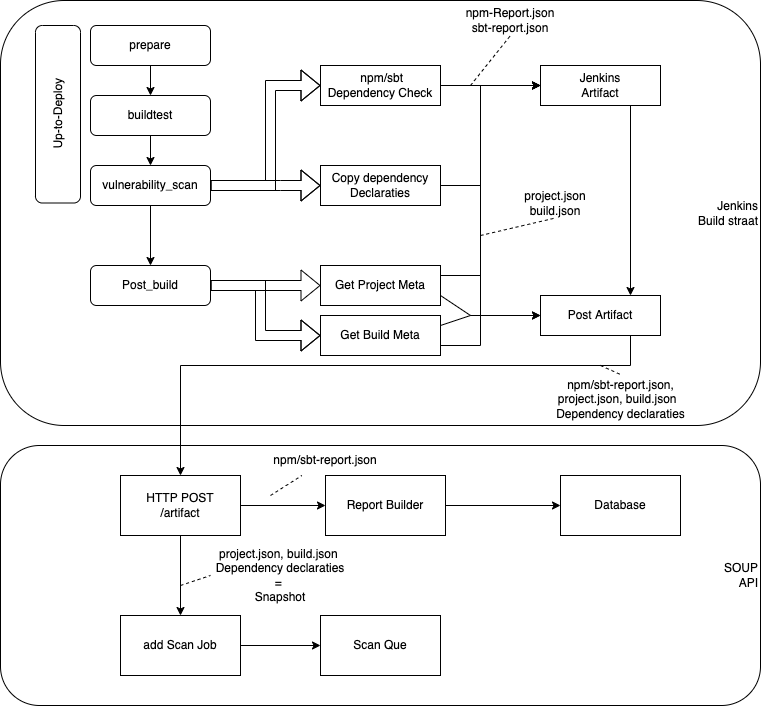
\includegraphics[width=15cm]{gfx/methode_Jenkins}
    \caption{Methode SOUP analyse}
    \label{fig:methodeSOUPanalyse}
\end{figure}

\subsection{Resultaat}\label{subsec:resultaat}
Door in de buildstraat te scannen wordt er een rapport ten tijde van de build gegenereerd. Ondanks dat dit de duur van de deploy kan verlengen wordt er hierdoor gegarandeerd dat er een rapport beschikbaar is over de uitgerolde externe bibliotheken. Door in dezelfde stap ook alle in het project aanwezige declaraties beschikbaar te stellen voor de SOUP API kan er op basis van die declaraties periodiek een analyse worden uitgevoerd. Door zowel de resultaten van de dependency check als de dependency declaraties waar deze check op is uitgevoerd veilig te stellen weet je zeker dat de periodieke scans dezelfde basis hebben als de tijdens de deploy uitgevoerde scan. De methode voor het periodiek scannen geeft de mogelijkheid om te scannen tijdens voor de server rustige momenten. Hierdoor is er minder impact van de SOUP-analyse op de performance tijdens kantooruren.
%TODO Hier goede plek?
Hoewel deze methode specifiek voor SBT en NPM projecten is uitgewerkt is er de wens om op een later stadium ook andere talen en platformen(Docker) toe te voegen. Echter op het moment dat er een tool kan worden gevonden die kwetsbaarheden op kan sporen in deze talen en of platformen waarbij een output kan worden gegenereerd op een zelfde manier als de hier beschreven tools. Dan zou er alleen een extra plugin moet worden geschreven die in de SOUP API die met deze data overweg kan om op die manier toch een uniforme data structuur te kunnen hanteren.

\subsection{Conclusie}\label{subsec:conclusie}
De hierboven genoemde methode maakt het in theorie mogelijk om middels een dependency check geautomatiseerd een SOUP-analyse uit te voeren tijdens de uitrol van een project, met als resultaat een rapport over de eventueel gevonden kwetsbaarheden. Tijdens de methode worden de projectgegevens veilig gesteld waardoor later op periodieke basis dezelfde dependency check kan worden uitgevoerd.
Deze methode maakt het mogelijk om inzichten te krijgen zodat de preventie stappen beschreven in OWASP top 10 - A06:2021 $"$Vulnerable and outdated components$"$ kunnen worden nageleefd.


\section{Eindconclusie}\label{sec:Eindconclusie}
In dit hoofdstuk zijn een aantal onderzoeken uitgevoerd. Deze hebben inzichten opgeleverd over hoe Eaglescience software ontwikkeld, waarbij aandacht is besteed aan de dev-stack, werkwijze en tooling. Deze bevindingen vormden de basis voor de zoektocht naar compatibele tooling voor SOUP analyses binnen Scala en TypeScript projecten, waarbij SBT en NPM worden gebruikt als buildtools. Doordat Eaglescience ontwikkeld in een 'niche-taal' (Scala) is de beschikbare tooling gelimiteerd. Desondanks is er voor beide door Eaglescience gebruikte hoofdtalen geschikte tooling gevonden om SOUP analyses mee uit te voeren (OWASP-dependency-check voor NPM en sbt-dependency-check voor SBT). Uit documentatie van deze tooling bleek dat er testen mee konden worden uitgevoerd om te onderzoeken hoe ze in een methode zouden kunnen worden geïmplementeerd om aan de project eisen te kunnen voldoen. De geselecteerde tooling bleken compatibel en goed te werken tijdens een reeks testen, en te voldoen aan de in de opdracht gestelde eisen. Tijdens deze testen werd inspiratie opgedaan voor een methode om gegevens uit de Jenskins buildstraat te verkrijgen en te analyseren. Door samenvoeging van de twee testmethodes is er een methode gevonden voor de analyse van externe bibliotheken binnen Eaglescience projecten. Deze methode maakt het in theorie mogelijk om zowel na deploy geautomatiseerd te draaien als op periodieke basis. Echter is de methode die is beschreven geschikt voor SBT en NPM projecten. Het doel is dat de output uit de buildstraat opgepikt moet kunnen worden door de API die vervolgens verantwoordelijk is voor het verwerken van de rauwe data in een gewenst formaat. Ieder platform dat wordt toegevoegd aan de SOUP analyse heeft dus een eigen SCA tool nodig met daarbij een passende plugin die de data van deze tool omzet naar het datamodel dat wordt gehanteerd binnen de API. De bevindingen van dit hoofdstuk zullen als basis dienen voor het ontwerp van de daadwerkelijke module voor de uitvoering van SOUP analyses.

%TODO Referentie naar datamodel van deze tool in bijlage?
